\documentclass[conference]{IEEEtran}
% \IEEEoverridecommandlockouts
% The preceding line is only needed to identify funding in the first footnote. If that is unneeded, please comment it out.
\usepackage{cite}
\usepackage{amsmath,amssymb,amsfonts}
\usepackage{algorithmic}
\usepackage{graphicx}
\usepackage{textcomp}
\usepackage{xcolor}
\def\BibTeX{{\rm B\kern-.05em{\sc i\kern-.025em b}\kern-.08em
    T\kern-.1667em\lower.7ex\hbox{E}\kern-.125emX}}
\begin{document}

\title{Development of Deep Q-Learning Agent for Playing the Game of Snake}
\author{\IEEEauthorblockN{1\textsuperscript{st} Guilherme G. Kowalczuk}
\IEEEauthorblockA{\textit{Instituto Tecnológico de Aeronáutica}\\
São José dos Campos, Brazil\\
guilherme.kowalczuk@ga.ita.br}
\and
\IEEEauthorblockN{2\textsuperscript{nd} Jian L. B. Veras}
\IEEEauthorblockA{\textit{Instituto Tecnológico de Aeronáutica}\\
São José dos Campos, Brazil\\
jian.veras@ga.ita.br}
\and
\IEEEauthorblockN{3\textsuperscript{rd} Rina C. Carvalho}
\IEEEauthorblockA{\textit{Instituto Tecnológico de Aeronáutica}\\
São José dos Campos, Brazil\\
rina.carvalho@ga.ita.br}
}

\maketitle


%%%%%%%%%%%%%%%%%%%%%%%%%%%%%%%%%%%%%%%%%%%%%%%%%%%%%%%%%%%%%%%%%%%%%%%%%%%%%%%%
\begin{abstract}

% This electronic document is a ÒliveÓ template. The various components of your paper [title, text, heads, etc.] are already defined on the style sheet, as illustrated by the portions given in this document.

This work presents the implementation of an agent for the game of Snake using Deep Q-Learning. We present the model, state space and reward engineering adopted, as well as the evolution of the agent's performance across training episodes and during evaluation. In this context, the trained agent is consistently capable of scoring at least 10 times per game in 70\% of its games. Lastly, we discuss the results and present conclusions regarding the employed methodology.

\end{abstract}


\section{INTRODUCTION}

First deep learning model to successfully learn control policies from high-dimensional sensory input using Reinforcement Learning (RL) was introduced by DeepMind in 2013. In that paper, they combined classical Deep Learning (DL) algorithms with RL to create a single, general-purpose learning agent that could learn directly from the screen input. The agent was able to learn to play seven Atari 2600 games by only observing the screen pixels and receiving a reward when the game score increased. This study was revolutionary since the agent was able to outperform all previous approaches on six of the games and surpassed a human expert on three of them.

Although Atari was high popular for Millennials and Gen X, the early Gen Z are more familiar with mobile games. One of them is the Snake game, usually played in a Nokia mobile. The game consists of a snake that moves around the screen and increases its score by eating apples and growing in length. The game ends when the snake collides with the borders of the screen or with its own body. The objective of the game is to obtain the highest score possible, which means survive and eat as many apples as possible, without eating its own body. The game of Snake is a good candidate for RL because it is a simple game with a clear reward function and a small state space. Figure \ref{snake-game} shows a illustration of the game.

\begin{figure}[thpb]
   \centering
%    \framebox{\parbox{3in}{We suggest that you use a text box to insert a graphic (which is ideally a 300 dpi TIFF or EPS file, with all fonts embedded) because, in an document, this method is somewhat more stable than directly inserting a picture.
% }}
   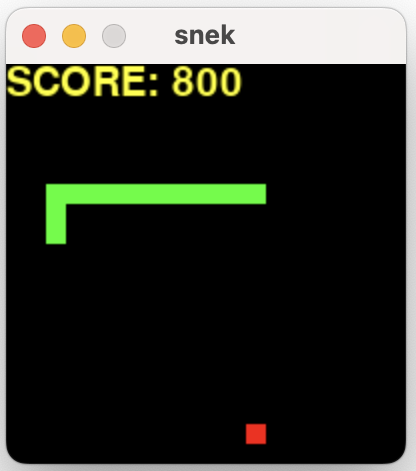
\includegraphics[scale=0.5]{snake-2.png}
   \caption{Snake game from a $20\times20$ grid wall. The main goal for the snake is to eat the apples without eating itself.}
   \label{snake-game}
\end{figure}

In this work, we present the implementation of an agent for the game of Snake using the Deep Q-Learning framework adopted by DeepMind. The main goal is to set up an simulation of the game and train an agent to play it. We present two forms for a state representation and discuss the results obtained by the agent.

\section{DEEP Q-LEARNING}

The Deep Q-Learning algorithm is a combination of Q-Learning and Deep Neural Networks (DNN). Q-Learning is a model-free RL algorithm that learns a policy by directly approximating the optimal action-value function $Q^*(s,a)$, which is the expected return for taking action $a$ in state $s$ and following the optimal policy thereafter. This is necessary because the problem may have too much states, so it's impossible (or really inefficient) to store the action-value function for all discrete state space.


\section{METHODOLOGY}

We developed the "Game of Snake" using PyGame, NumPy, Collections in Python. The game architecture is based on three classes: the \texttt{Grid}, which corresponds to the space where the game occurs and also houses the apple (the target for the agent); the \texttt{Agent}, which represents the snake; and the \texttt{Game}, which orchestrates the interactions between the agent and the environment.

There are two game modes: one with closed walls, and the other without. In the first mode, the game-over event happens when the agent touches the borders of the window. However, this event does not occur in the second mode. Another way for the game to end is when the snake's head collides with its body, in both modes. The score increases every time the agent obtains the target (the apple), and a new target is randomly created afterward.

We used Keras to implement the deep neural network, which evaluate the action values. The architecture consists on four dense layers, as presented in Table \ref{tab:NNarchtecture}



\subsection{Deep Q-Learning}

O QUE É? COMO FUNCIONA? QUAL A REDE IMPLEMENTADA? \textbf{POR QUE OS CACHORROS LAMBEM O PRÓPRIO KOO? E O \textit{GAYS} LAMBEM O koo ALHEIO????}

\subsection{Experience Replay}

MECANISMO

\subsection{Fixed Q-Targets}

MAIS BLÁBLÁBLÁ

\subsection{Reward Engineering} 

ATOLA LINGUIÇA

\subsection{Units}

\begin{itemize}

\item Use either SI (MKS) or CGS as primary units. (SI units are encouraged.) English units may be used as secondary units (in parentheses). An exception would be the use of English units as identifiers in trade, such as Ò3.5-inch disk driveÓ.
\item Avoid combining SI and CGS units, such as current in amperes and magnetic field in oersteds. This often leads to confusion because equations do not balance dimensionally. If you must use mixed units, clearly state the units for each quantity that you use in an equation.
\item Do not mix complete spellings and abbreviations of units: ÒWb/m2Ó or Òwebers per square meterÓ, not Òwebers/m2Ó.  Spell out units when they appear in text: Ò. . . a few henriesÓ, not Ò. . . a few HÓ.
\item Use a zero before decimal points: Ò0.25Ó, not Ò.25Ó. Use Òcm3Ó, not ÒccÓ. (bullet list)

\end{itemize}


\subsection{Equations}

The equations are an exception to the prescribed specifications of this template. You will need to determine whether or not your equation should be typed using either the Times New Roman or the Symbol font (please no other font). To create multileveled equations, it may be necessary to treat the equation as a graphic and insert it into the text after your paper is styled. Number equations consecutively. Equation numbers, within parentheses, are to position flush right, as in (1), using a right tab stop. To make your equations more compact, you may use the solidus ( / ), the exp function, or appropriate exponents. Italicize Roman symbols for quantities and variables, but not Greek symbols. Use a long dash rather than a hyphen for a minus sign. Punctuate equations with commas or periods when they are part of a sentence, as in

$$
\alpha + \beta = \chi \eqno{(1)}
$$

Note that the equation is centered using a center tab stop. Be sure that the symbols in your equation have been defined before or immediately following the equation. Use Ò(1)Ó, not ÒEq. (1)Ó or Òequation (1)Ó, except at the beginning of a sentence: ÒEquation (1) is . . .Ó

\subsection{Some Common Mistakes}
\begin{itemize}


\item The word ÒdataÓ is plural, not singular.
\item The subscript for the permeability of vacuum ?0, and other common scientific constants, is zero with subscript formatting, not a lowercase letter ÒoÓ.
\item In American English, commas, semi-/colons, periods, question and exclamation marks are located within quotation marks only when a complete thought or name is cited, such as a title or full quotation. When quotation marks are used, instead of a bold or italic typeface, to highlight a word or phrase, punctuation should appear outside of the quotation marks. A parenthetical phrase or statement at the end of a sentence is punctuated outside of the closing parenthesis (like this). (A parenthetical sentence is punctuated within the parentheses.)
\item A graph within a graph is an ÒinsetÓ, not an ÒinsertÓ. The word alternatively is preferred to the word ÒalternatelyÓ (unless you really mean something that alternates).
\item Do not use the word ÒessentiallyÓ to mean ÒapproximatelyÓ or ÒeffectivelyÓ.
\item In your paper title, if the words Òthat usesÓ can accurately replace the word ÒusingÓ, capitalize the ÒuÓ; if not, keep using lower-cased.
\item Be aware of the different meanings of the homophones ÒaffectÓ and ÒeffectÓ, ÒcomplementÓ and ÒcomplimentÓ, ÒdiscreetÓ and ÒdiscreteÓ, ÒprincipalÓ and ÒprincipleÓ.
\item Do not confuse ÒimplyÓ and ÒinferÓ.
\item The prefix ÒnonÓ is not a word; it should be joined to the word it modifies, usually without a hyphen.
\item There is no period after the ÒetÓ in the Latin abbreviation Òet al.Ó.
\item The abbreviation Òi.e.Ó means Òthat isÓ, and the abbreviation Òe.g.Ó means Òfor exampleÓ.

\end{itemize}


\section{USING THE TEMPLATE}

Use this sample document as your LaTeX source file to create your document. Save this file as {\bf root.tex}. You have to make sure to use the cls file that came with this distribution. If you use a different style file, you cannot expect to get required margins. Note also that when you are creating your out PDF file, the source file is only part of the equation. {\it Your \TeX\ $\rightarrow$ PDF filter determines the output file size. Even if you make all the specifications to output a letter file in the source - if your filter is set to produce A4, you will only get A4 output. }

It is impossible to account for all possible situation, one would encounter using \TeX. If you are using multiple \TeX\ files you must make sure that the  source file is called root.tex - this is particularly important if your conference is using PaperPlaza's built in \TeX\ to PDF conversion tool.

\subsection{Headings, etc}

Text heads organize the topics on a relational, hierarchical basis. For example, the paper title is the primary text head because all subsequent material relates and elaborates on this one topic. If there are two or more sub-topics, the next level head (uppercase Roman numerals) should be used and, conversely, if there are not at least two sub-topics, then no subheads should be introduced. Styles named ÒHeading 1Ó, ÒHeading 2Ó, ÒHeading 3Ó, and ÒHeading 4Ó are prescribed.

\subsection{Figures and Tables}

Positioning Figures and Tables: Place figures and tables at the top and bottom of columns. Avoid placing them in the middle of columns. Large figures and tables may span across both columns. Figure captions should be below the figures; table heads should appear above the tables. Insert figures and tables after they are cited in the text. Use the abbreviation ÒFig. 1Ó, even at the beginning of a sentence.

\begin{table}[h]
\caption{An Example of a Table}
\label{table_example}
\begin{center}
\begin{tabular}{|c||c|}
\hline
One & Two\\
\hline
Three & Four\\
\hline
\end{tabular}
\end{center}
\end{table}


   \begin{figure}[thpb]
      \centering
      \framebox{\parbox{3in}{We suggest that you use a text box to insert a graphic (which is ideally a 300 dpi TIFF or EPS file, with all fonts embedded) because, in an document, this method is somewhat more stable than directly inserting a picture.
}}
      %\includegraphics[scale=1.0]{figurefile}
      \caption{Inductance of oscillation winding on amorphous
       magnetic core versus DC bias magnetic field}
      \label{figurelabel}
   \end{figure}
   

Figure Labels: Use 8 point Times New Roman for Figure labels. Use words rather than symbols or abbreviations when writing Figure axis labels to avoid confusing the reader. As an example, write the quantity ÒMagnetizationÓ, or ÒMagnetization, MÓ, not just ÒMÓ. If including units in the label, present them within parentheses. Do not label axes only with units. In the example, write ÒMagnetization (A/m)Ó or ÒMagnetization {A[m(1)]}Ó, not just ÒA/mÓ. Do not label axes with a ratio of quantities and units. For example, write ÒTemperature (K)Ó, not ÒTemperature/K.Ó

\section{CONCLUSIONS}

A conclusion section is not required. Although a conclusion may review the main points of the paper, do not replicate the abstract as the conclusion. A conclusion might elaborate on the importance of the work or suggest applications and extensions. 

\addtolength{\textheight}{-12cm}   % This command serves to balance the column lengths
                                  % on the last page of the document manually. It shortens
                                  % the textheight of the last page by a suitable amount.
                                  % This command does not take effect until the next page
                                  % so it should come on the page before the last. Make
                                  % sure that you do not shorten the textheight too much.

%%%%%%%%%%%%%%%%%%%%%%%%%%%%%%%%%%%%%%%%%%%%%%%%%%%%%%%%%%%%%%%%%%%%%%%%%%%%%%%%



%%%%%%%%%%%%%%%%%%%%%%%%%%%%%%%%%%%%%%%%%%%%%%%%%%%%%%%%%%%%%%%%%%%%%%%%%%%%%%%%



%%%%%%%%%%%%%%%%%%%%%%%%%%%%%%%%%%%%%%%%%%%%%%%%%%%%%%%%%%%%%%%%%%%%%%%%%%%%%%%%
\section*{APPENDIX}

Appendixes should appear before the acknowledgment.

\section*{ACKNOWLEDGMENT}

The preferred spelling of the word ÒacknowledgmentÓ in America is without an ÒeÓ after the ÒgÓ. Avoid the stilted expression, ÒOne of us (R. B. G.) thanks . . .Ó  Instead, try ÒR. B. G. thanksÓ. Put sponsor acknowledgments in the unnumbered footnote on the first page.



%%%%%%%%%%%%%%%%%%%%%%%%%%%%%%%%%%%%%%%%%%%%%%%%%%%%%%%%%%%%%%%%%%%%%%%%%%%%%%%%

References are important to the reader; therefore, each citation must be complete and correct. If at all possible, references should be commonly available publications.



\begin{thebibliography}{99}
\bibitem{Sebastianelli} A. Sebastianelli, M. Tipaldi, S. L. Ullo and L. Glielmo, "A Deep Q-Learning based approach applied to the Snake game," 2021 29th Mediterranean Conference on Control and Automation (MED), PUGLIA, Italy, 2021, pp. 348-353, doi: 10.1109/MED51440.2021.9480232.

\end{thebibliography}




\end{document}
